\begin{figure}[tb]
\centering
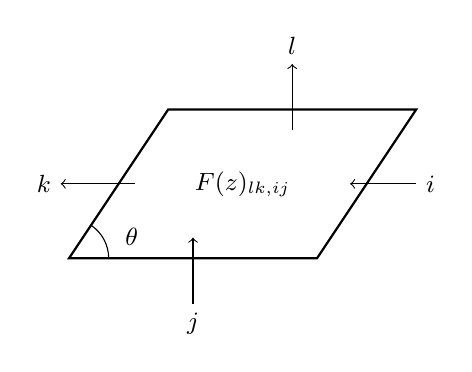
\begin{tikzpicture}[scale=1.05,every node/.style={font=\small}]
 \draw[thick] (0,0)--(3,0)--(4.2,1.8)--(1.2,1.8)--cycle;
 \draw[->] (4.2,.9)--(3.4,.9);
 \draw[->] (.8,.9)--(-.1,.9);
 \draw[->] (1.5,-.55)--(1.5,.25);
 \draw[->] (2.7,1.55)--(2.7,2.35);
 \node[right] at (4.2,.9) {$i$};
 \node[left] at (-.1,.9) {$k$};
 \node[below] at (1.5,-.55) {$j$};
 \node[above] at (2.7,2.35) {$l$};
 \draw (.48,0) arc[start angle=0,end angle=56.31,radius=.48];
 \node at (.76,.26) {$\theta$};
 \node at (2.1,.9) {$F(z)_{lk,ij}$};
\end{tikzpicture}
\caption{Port and tensor order for the checked rhombus matrix.
The horizontal stream enters at the right and leaves at the left;
the vertical stream enters below and leaves above. The arrows specify
the positive spin directions, not a particular allowed path pairing.
The local phase convention is imposed on each pairing separately.}
\label{fig:pv:row}
\end{figure}
